\documentclass[tikz,border=6pt]{standalone}
\usepackage{tikz}
\usetikzlibrary{arrows.meta,positioning,backgrounds}

\begin{document}
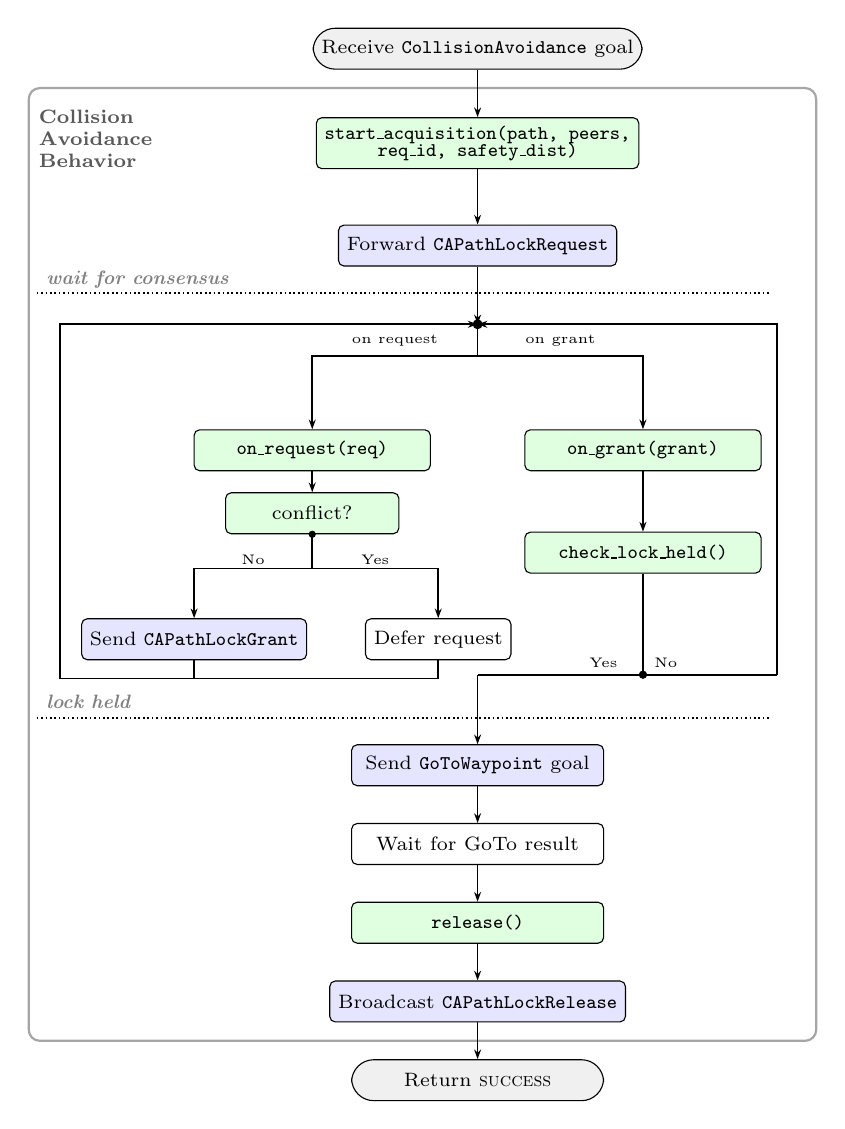
\begin{tikzpicture}[
  font=\scriptsize,
  term/.style={draw, rounded corners=8pt, fill=black!6,
               minimum width=3.2cm, minimum height=0.52cm,
               align=center, inner sep=3pt, text=black},
  pstep/.style={draw, rounded corners=2pt, fill=green!12,
                minimum width=3.2cm, minimum height=0.52cm,
                align=center, inner sep=3pt, text=black},
  pbstep/.style={draw, rounded corners=2pt, fill=green!12,
                minimum width=3.0cm, minimum height=0.52cm,
                align=center, inner sep=3pt, text=black},
  sstep/.style={draw, rounded corners=2pt, fill=blue!10,
                minimum width=3.2cm, minimum height=0.52cm,
                align=center, inner sep=3pt, text=black},
  sbstep/.style={draw, rounded corners=2pt, fill=blue!10,
                minimum width=3.0cm, minimum height=0.52cm,
                align=center, inner sep=3pt, text=black},
  lstep/.style={draw, rounded corners=2pt, fill=white,
                minimum width=3.2cm, minimum height=0.52cm,
                align=center, inner sep=3pt, text=black},
  lbstep/.style={draw, rounded corners=2pt, fill=white,
                minimum width=3.0cm, minimum height=0.52cm,
                align=center, inner sep=3pt, text=black},
  arr/.style={-{Stealth[length=3.5pt,width=2.5pt]}, semithick},
  back/.style={semithick, black},
  lbl/.style={font=\tiny},
  sep/.style={densely dotted, black, semithick},
  phase/.style={font=\scriptsize\bfseries\itshape, black!50},
]

  \def\fc{0}
  \def\lb{-2.1}
  \def\rb{2.1}

  % Phase 1 — Lock request

  \node[term]  (start) at (\fc, 0.00)
    {Receive \texttt{CollisionAvoidance} goal};

  \node[pstep] (acq)   at (\fc, -1.20)
    {\texttt{start\_acquisition(path, peers,}\\[-2pt]
     \texttt{req\_id, safety\_dist)}};

  \node[sstep] (freq)  at (\fc, -2.50)
    {Forward \texttt{CAPathLockRequest}};


  \draw[sep] (-5.6,-3.10) -- (3.7,-3.10);
  \node[phase, anchor=west] at (-5.6,-2.93) {wait for consensus};

  % Phase 2 — Lock negotiation (two branches, loop)

  % Junction where loop-backs re-enter, and fork below it
  \coordinate (looptop) at (0, -3.50);
  \coordinate (fork)    at (0, -3.90);

  % Left branch: on_request → conflict decision → grant or defer
  \node[pbstep] (preq)   at (\lb, -5.10) {\texttt{on\_request(req)}};
  \node[pbstep, minimum width=2.2cm] (conf) at (\lb, -5.90) {conflict?};
  \node[sbstep, minimum width=2.0cm] (sgrant) at (-3.6, -7.50) {Send \texttt{CAPathLockGrant}};
  \node[lbstep, minimum width=1.8cm] (defer) at (-0.5, -7.50) {Defer request};

  % Right branch: on_grant
  \node[pbstep] (ogrant) at (\rb, -5.10) {\texttt{on\_grant(grant)}};
  \node[pbstep] (chk)    at (\rb, -6.40) {\texttt{check\_lock\_held()}};


  \draw[sep] (-5.6,-8.5) -- (3.7,-8.5);
  \node[phase, anchor=west] at (-5.6,-8.3) {lock held};

  % Phase 3 — Execution and release

  \node[sstep] (goto)   at (\fc, -9.10)  {Send \texttt{GoToWaypoint} goal};
  \node[lstep] (waitgo) at (\fc, -10.10) {Wait for GoTo result};
  \node[pstep] (rel)    at (\fc, -11.10) {\texttt{release()}};
  \node[sstep] (brel)   at (\fc, -12.10) {Broadcast \texttt{CAPathLockRelease}};
  \node[term]  (done)   at (\fc, -13.10) {Return \textsc{success}};

  % Arrows — Phase 1

  \draw[arr] (start.south) -- (acq.north);
  \draw[arr] (acq.south)   -- (freq.north);

  % freq → junction (looptop) → fork
  \draw[arr] (freq.south)  -- (looptop);
  \draw      (looptop)     -- (fork);
  \fill      (looptop) circle (1.8pt);

  % Arrows — Phase 2 branches

  % Fork → left branch
  \draw[arr] (fork) -- (\lb,-3.90) -- (preq.north);
  \node[lbl, anchor=south] at ({(\fc+\lb)/2},-3.90) {on request};

  % Fork → right branch
  \draw[arr] (fork) -- (\rb,-3.90) -- (ogrant.north);
  \node[lbl, anchor=south] at ({(\fc+\rb)/2},-3.90) {on grant};

  % preq → conflict decision → grant or defer
  \draw[arr] (preq.south) -- (conf.north);
  \fill (conf.south) circle (1.3pt);
  \draw[arr] (conf.south) -- (\lb,-6.60) -- (-3.6,-6.60) -- (sgrant.north);
  \node[lbl, anchor=south] at (-2.85,-6.68) {No};
  \draw[arr] (conf.south) -- (\lb,-6.6) -- (-0.5,-6.6) -- (defer.north);
  \node[lbl, anchor=south] at (-1.30,-6.68) {Yes};

  \draw[arr] (ogrant.south) -- (chk.north);

  % Left loop-backs: sgrant and defer feed into left spine
  \draw[back] (sgrant.south) -- (-3.6,-8) -- (-5.3,-8);
  \draw[back] (defer.south)  -- (-0.5,-8) -- (-5.3,-8);

  % Left spine (shared): carries all loop-backs up to looptop
  \draw[arr] (-5.3,-8) -- (-5.3,-3.50) -- (looptop);

  % chk.south → junction dot for No / Yes split
  \draw[back] (chk.south) -- (\rb,-7.95);
  \fill (\rb,-7.95) circle (1.5pt);

  % No: turn right, go up, return to looptop from the right
  \draw[back] (\rb,-7.95) -- (3.8,-7.95);
  \draw[arr]  (3.8,-7.95) -- (3.8,-3.50) -- (looptop);
  \node[lbl, anchor=west] at (2.12,-7.80) {No};

  % Arrows — Phase 2 → Phase 3 (Yes)

  \draw[back] (\rb,-7.95) -- (\rb,-7.95) -- (0,-7.95);
  \draw[arr]  (0,-7.95)   -- (goto.north);
  \node[lbl, anchor=east] at (1.90,-7.80) {Yes};

  % Arrows — Phase 3

  \draw[arr] (goto.south)   -- (waitgo.north);
  \draw[arr] (waitgo.south) -- (rel.north);
  \draw[arr] (rel.south)    -- (brel.north);
  \draw[arr] (brel.south)   -- (done.north);

  % Bounding box
  \begin{scope}[on background layer]
    \draw[rounded corners=4pt, black!35, thick]
      (-5.7, -0.5) rectangle (4.3, -12.6);
    \node[font=\scriptsize\bfseries, text=black!65, fill=white, inner sep=2pt,
          anchor=north west, align=left] at (-5.65,-0.7)
      {Collision\\Avoidance\\Behavior};
  \end{scope}

  % Legend
  % \node[pstep, minimum width=1.6cm, minimum height=0.38cm, inner sep=1pt,
        font=\tiny] at (-3.2,-10.80) {plugin call};
  % \node[sstep, minimum width=1.6cm, minimum height=0.38cm, inner sep=1pt,
        font=\tiny] at (-3.2,-11.50) {CAGateway};
  % \node[lstep, minimum width=1.6cm, minimum height=0.38cm, inner sep=1pt,
        font=\tiny] at (-3.2,-12.20) {behavior logic};

\end{tikzpicture}
\end{document}
